% !TEX TS-program = XeLaTeX
% use the following command:
% all document files must be coded in UTF-8
\documentclass[spanish]{textolivre}
% build HTML with: make4ht -e build.lua -c textolivre.cfg -x -u article "fn-in,svg,pic-align"

\journalname{Texto Livre}
\thevolume{15}
%\thenumber{1} % old template
\theyear{2022}
\receiveddate{\DTMdisplaydate{2022}{1}{10}{-1}} % YYYY MM DD
\accepteddate{\DTMdisplaydate{2022}{3}{8}{-1}}
\publisheddate{\DTMdisplaydate{2022}{5}{17}{-1}}
\corrauthor{María del Rosario Neira-Piñeiro}
\articledoi{10.35699/1983-3652.2022.37844}
%\articleid{NNNN} % if the article ID is not the last 5 numbers of its DOI, provide it using \articleid{} commmand 
% list of available sesscions in the journal: articles, dossier, reports, essays, reviews, interviews, editorial
\articlesessionname{articles}
\runningauthor{Del-Moral Pérez et al.} 
%\editorname{Leonardo Araújo} % old template
\sectioneditorname{Hugo Heredia Ponce}
\layouteditorname{Leonado Araújo}

\title{Aprendizaje autorregulado del alumnado de Educación Infantil al narrar historias orales con una app}
\othertitle{Aprendizagem autorregulada de alunos da educação infantil ao contar histórias orais com aplicativo}
\othertitle{Self-regulated learning of early childhood education students making oral storytelling with an app}
% if there is a third language title, add here:
%\othertitle{Artikelvorlage zur Einreichung beim Texto Livre Journal}

\author[1]{María Esther Del-Moral Pérez~\orcid{0000-0002-9143-5960}~\thanks{Email: \url{emoral@uniovi.es}}}
\author[1]{Nerea López-Bouzas~\orcid{0000-0003-0753-0672}~\thanks{Email: \url{lopeznerea@uniovi.es}}}
\author[1]{Jonathan Castañeda Fernández~\orcid{0000-0003-4934-2979}~\thanks{Email: \url{castanedajonathan@uniovi.es}}}
\author[1]{María del Rosario Neira-Piñeiro~\orcid{0000-0003-2355-4682}~\thanks{Email: \url{neiramaria@uniovi.es}}}
\affil[1]{Universidad de Oviedo, Facultad de Formación del Profesorado y Educación, Departamento de Ciencias de la Educación, Oviedo, España.}

\addbibresource{article.bib}
% use biber instead of bibtex
% $ biber article

% used to create dummy text for the template file
\definecolor{dark-gray}{gray}{0.35} % color used to display dummy texts
\usepackage{lipsum}
\SetLipsumParListSurrounders{\colorlet{oldcolor}{.}\color{dark-gray}}{\color{oldcolor}}

% used here only to provide the XeLaTeX and BibTeX logos
\usepackage{hologo}

% if you use multirows in a table, include the multirow package
\usepackage{multirow}

% provides sidewaysfigure environment
\usepackage{rotating}

% CUSTOM EPIGRAPH - BEGIN 
%%% https://tex.stackexchange.com/questions/193178/specific-epigraph-style
\usepackage{epigraph}
\renewcommand\textflush{flushright}
\makeatletter
\newlength\epitextskip
\pretocmd{\@epitext}{\em}{}{}
\apptocmd{\@epitext}{\em}{}{}
\patchcmd{\epigraph}{\@epitext{#1}\\}{\@epitext{#1}\\[\epitextskip]}{}{}
\makeatother
\setlength\epigraphrule{0pt}
\setlength\epitextskip{0.5ex}
\setlength\epigraphwidth{.7\textwidth}
% CUSTOM EPIGRAPH - END

% LANGUAGE - BEGIN
% ARABIC
% for languages that use special fonts, you must provide the typeface that will be used
% \setotherlanguage{arabic}
% \newfontfamily\arabicfont[Script=Arabic]{Amiri}
% \newfontfamily\arabicfontsf[Script=Arabic]{Amiri}
% \newfontfamily\arabicfonttt[Script=Arabic]{Amiri}
%
% in the article, to add arabic text use: \textlang{arabic}{ ... }
%
% RUSSIAN
% for russian text we also need to define fonts with support for Cyrillic script
% \usepackage{fontspec}
% \setotherlanguage{russian}
% \newfontfamily\cyrillicfont{Times New Roman}
% \newfontfamily\cyrillicfontsf{Times New Roman}[Script=Cyrillic]
% \newfontfamily\cyrillicfonttt{Times New Roman}[Script=Cyrillic]
%
% in the text use \begin{russian} ... \end{russian}
% LANGUAGE - END

% EMOJIS - BEGIN
% to use emoticons in your manuscript
% https://stackoverflow.com/questions/190145/how-to-insert-emoticons-in-latex/57076064
% using font Symbola, which has full support
% the font may be downloaded at:
% https://dn-works.com/ufas/
% add to preamble:
% \newfontfamily\Symbola{Symbola}
% in the text use:
% {\Symbola }
% EMOJIS - END

% LABEL REFERENCE TO DESCRIPTIVE LIST - BEGIN
% reference itens in a descriptive list using their labels instead of numbers
% insert the code below in the preambule:
%\makeatletter
%\let\orgdescriptionlabel\descriptionlabel
%\renewcommand*{\descriptionlabel}[1]{%
%  \let\orglabel\label
%  \let\label\@gobble
%  \phantomsection
%  \edef\@currentlabel{#1\unskip}%
%  \let\label\orglabel
%  \orgdescriptionlabel{#1}%
%}
%\makeatother
%
% in your document, use as illustraded here:
%\begin{description}
%  \item[first\label{itm1}] this is only an example;
%  % ...  add more items
%\end{description}
% LABEL REFERENCE TO DESCRIPTIVE LIST - END


% add line numbers for submission
%\usepackage{lineno}
%\linenumbers

\usepackage{siunitx}
\sisetup{output-decimal-marker={,}}

\begin{document}
\maketitle

\begin{polyabstract}
\begin{abstract}
Este estudio analiza el nivel de autorregulación -a partir de las dimensiones de autonomía y reacción afectivo-emocional- del alumnado de Educación Infantil ($N=93$) durante tareas narrativas apoyadas en la app Imagistory, creadora de relatos. Para ello, se adoptó una metodología mixta: cualitativa, mediante la observación sistemática, atendiendo a dos dimensiones durante el proceso narrativo, y cuantitativa de carácter no experimental, descriptivo y correlacional. Entre los resultados se constata que, independientemente del género, edad y uso de tabletas, la autonomía del aprendizaje y la reacción afectiva se incrementan durante la tarea narrativa apoyada en la app. Sin embargo, la extroversión y el nivel de destreza con la app se relacionan con el aumento de la autonomía y reacción afectiva del alumnado. Las experiencias mediadas por app pueden ser enriquecedoras en esta etapa, pues contribuyen a la autorregulación del aprendizaje del alumnado al incrementar su autonomía y espontaneidad para acometer tareas narrativas, al tiempo que favorecen la competencia comunicativa mediante la expresión oral apoyada en ilustraciones y estimulan la competencia digital y la alfabetización visual. Asimismo, la narración mediada con app les ofrece la oportunidad de expresar sus emociones, empatizar con personajes, incrementar su interés, curiosidad, seguridad y disfrute, al implicarse en la historia.

\keywords{App \sep Relatos digitales \sep Educación Infantil \sep Aprendizaje autorregulado \sep Narración oral}
\end{abstract}

\begin{portuguese}
\begin{abstract}
Este estudo analisa o nível de autorregulação - a partir da dimensão da autonomia e reação afetivo-emocional - de alunos da Educação Infantil ($N=93$) durante tarefas narrativas apoiadas pelo aplicativo Imagistory, que cria histórias. Para tanto, foi adotada uma metodologia mista: qualitativa, por meio da observação sistemática atendendo a duas dimensões durante o processo narrativo; e quantitativa de caráter não experimental, descritivo e correlacional. Dentre os resultados, verifica-se que, independente do sexo, idade e uso de \textit{tablets}, a autonomia de aprendizagem e a reação afetiva aumentam durante a tarefa narrativa apoiada pelo aplicativo. No entanto, a extroversão e o nível de habilidade com o aplicativo estão relacionados ao aumento da autorregulação e da reação afetiva dos alunos. As experiências mediadas por aplicativos podem ser enriquecedoras nessa fase, pois contribuem para a autorregulação da aprendizagem do aluno, aumentando sua autonomia e espontaneidade para realizar tarefas narrativas, ao mesmo tempo em que promovem a competência comunicativa por meio da expressão oral apoiada em ilustrações, estimulando a competência digital e o letramento visual. Da mesma forma, a narrativa mediada por aplicativos oferece aos usuários a oportunidade de expressar suas emoções, ter empatia pelos personagens, aumentar seu interesse, curiosidade, segurança e diversão, envolvendo-se na história.

\keywords{Aplicativo \sep História digital \sep Educação Infantil \sep Autorregulação \sep Narração oral}
\end{abstract}
\end{portuguese}

\begin{english}
\begin{abstract}
This research analyses the level of self-regulation – based on  the autonomy and affective-emotional reaction  dimensions – of early childhood education students ($N=93$) doing narrative tasks supported by the story-creation app Imagistory. To do that, a mixed methodology was employed: qualitative, through the systematic observation with attention to 2 dimensions during the narrative process; and quantitative, with a non-experimental descriptive and correlational character. According to the results, it is observed that the autonomy in learning and the affective reaction increase during the narrative task supported by the app,  regardless of genre, age and tablets use. However, the extroversion and the skill level with the app are related to the increase of students’ self-regulation and affective reaction. The experiences with the app can be enriching at this educational level, as they contribute to  students’ learning self-regulation, increasing their autonomy and spontaneity to carry out narrative tasks. They also favor their communicative competence through oral expression based on illustrations and foster digital competence and visual literacy. Besides, the story supported by the app offers children the opportunity to express their emotions, empathize with the characters, and increase their interest, curiosity, security and enjoyment, as they get involved in the story.

\keywords{App \sep Digital storytelling \sep Early Childhood Education \sep Self-regulation \sep Oral storytelling}
\end{abstract}
\end{english}
% if there is another abstract, insert it here using the same scheme
\end{polyabstract}

\section{Introducción}\label{sec-intro}
Los estudios de \textcite{lisenbee_engaging_2018,neumann_use_2017,obyrne_digital_2018} subrayan que la utilización de aplicaciones digitales (app) con fines educativos en primeras edades se está generalizando de tal manera que la alfabetización digital de los menores está aumentando aceleradamente. Estas herramientas favorecen múltiples alfabetizaciones, claves en el siglo XXI. Asimismo, las experiencias formativas apoyadas en app de \textcite{abdel-reheem_amin_review_2020,camilleri_students_2019,rodriguez_digital_2021} arrojan resultados positivos ligados al incremento de la competencia lingüístico-narrativa, las habilidades lecto-escritoras y el aprendizaje de idiomas. \textcite{fu_exploring_2021} señalan que algunas app estimulan la producción oral del alumnado. Otras presentan relatos soportados en secuencias de imágenes que inducen la actividad intelectiva, proporcionando el andamiaje necesario para organizarlas e integrarlas en un discurso coherente, siguiendo la lógica operacional completa y asignándole un significado a la historia narrada. 

El componente lúdico e interactivo y los elementos audiovisuales, junto con el carácter inmersivo de estas herramientas, son factores que las dotan de gran motivación, siendo capaces de involucrar emocionalmente a los sujetos en actividades de aprendizaje al convertirlas en juego \cite{barton_immediate_2020,marsh_play_2018,strasser_towards_2015}. La potencialidad de las app para favorecer el \textit{engagement} de los usuarios con tareas como la lectura, la escritura o la narración se relaciona con su diseño intuitivo de carácter lúdico -cargado de incentivos sensoriales- que reduce el esfuerzo cognitivo que implica su realización \cite{ghalebandi_engaging_2019,tavernier_emerging_2020}.

Lógicamente, como indican \textcite{papadakis_educational_2018}, se precisa seleccionar las app atendiendo a los objetivos de aprendizaje que se desean alcanzar. \textcite{kay_creating_2018} las categoriza en app metacognitivas, constructivas, productivas y colaborativas, en tanto favorecen aprendizajes conceptuales y/o procedimentales, fomentan la construcción o elaboración de productos, o estimulan la colaboración. La evaluación de veinte app creadoras de relatos digitales -efectuada por \textcite{del-moral_evaluacion_2019}- identifica su potencial para promover la competencia comunicativa y la creatividad en Educación Infantil y Primaria. Estas app fomentan el aprendizaje por descubrimiento mediante la observación y la exploración, contribuyendo a impulsar la autorregulación del aprendizaje, entendida como la competencia que posibilita al alumnado activar sus propias estrategias para lograr los objetivos propuestos \cite{panadero_teorias_2014}. 


\section{Autorregulación del aprendizaje durante la producción oral de relatos a partir de aplicaciones digitales}\label{sec-autorregulacion}

El aprendizaje autorregulado se identifica con el comportamiento metacognitivo que permite a los sujetos activar estrategias funcionales para acometer una tarea \cite{hacker_metacognition_1998}. \textcite{kaplan_clarifying_2008} señala que la autorregulación no puede concebirse como un constructo único, pues se vincula con el modo en que la persona se sitúa frente al aprendizaje, lo que se asocia con el control metacognitivo \cite{winne_inherent_1995}. \textcite{alvarez_valdivia_evaluar_2009,berridi_ramirez_estrategias_2017} identifican cuatro fases en el proceso de autorregulación del aprendizaje: i) \textit{definición de la tarea}: establecimiento de las relaciones entre los conocimientos previos, intereses y motivaciones del sujeto, y los requerimientos cognitivos que conlleva su realización; ii) \textit{toma de decisiones}: definición de metas y acciones resolutivas de acuerdo con el tipo de tarea; iii) \textit{ejecución de las acciones}: compromiso con las estrategias elegidas e implementación de respuestas asociadas a las demandas; y iv) \textit{adaptación y evaluación}: ajuste de estrategias para lograr los objetivos planteados, reflexionando y autoevaluando el proceso y sus resultados.

Estas fases no son lineales, pues cada sujeto establece un ciclo en el que controla, ajusta y corrige sus aprendizajes, contribuyendo al desarrollo de sus funciones cognitivas \cite{colomina_observacion_1997}. El aprendizaje autorregulado refleja la autonomía de los sujetos para abordar una tarea con decisión y seguridad, así como su compromiso y deseo de realizarla, lo que se asocia con su motivación, es decir, con el interés que despierte y lo gratificante que resulte. Obviamente, docentes y recursos cobran gran importancia, pues pueden incrementar y favorecer la autorregulación del aprendizaje. En el contexto del aprendizaje narrativo, es esencial el papel de los agentes mediadores (docentes, adultos de la familia, etc.), y resultan clave en Educación Infantil \cite{torremocha_libros_2002}.

Desde edades tempranas, la creación de relatos constituye una actividad eficaz para potenciar la creatividad, la agilidad mental y los procesos cognitivos implicados en la narración de forma autónoma \cite{addone_engaging_2022}. En la actualidad, existen app digitales creadoras de relatos muy motivadoras, que favorecen el proceso de planificación y regulación de la tarea narrativa, logrando estimular las habilidades lingüístico-gramaticales y creativas de los escolares \cite{del-moral_aportaciones_2021}. Por su parte, \textcite{infante-villagran_aplicaciones_2021} constatan que la utilización de recursos digitales en niveles superiores de enseñanza activa procesos metacognitivos complejos e incrementa la motivación del alumnado, incidiendo en una mayor autorregulación de su aprendizaje.

Conscientes de que la elaboración de relatos estimula los procesos cognitivos al gestar una narración secuenciada, y que las app constituyen unos atractivos recursos interactivos para los escolares, la originalidad de este estudio -frente a las mencionadas investigaciones-, radica en constatar la contribución de una app creadora de relatos orales al incremento de la autorregulación del aprendizaje en Educación Infantil. Si bien existen estudios sobre el desarrollo de habilidades con app  \cite{abdel-reheem_amin_review_2020,rodriguez_digital_2021}, aquí se analiza su influencia en la autorregulación del aprendizaje a partir del nivel de autonomía del alumnado -antes y durante la tarea narrativa-, así como la reacción afectiva suscitada, utilizando un instrumento extrapolable a otros contextos. 


\section{Metodología}\label{sec-metodologia}

Se trata de un estudio no experimental, de tipo descriptivo y correlacional, de carácter mixto: a) \textit{cualitativo}, centrado en el análisis del nivel de autorregulación del aprendizaje del alumnado al crear un relato oral con una app, mediante la observación sistemática con un instrumento diseñado \textit{ad hoc}, previamente validado. Y, b) \textit{cuantitativo}, en relación con el tratamiento estadístico de los datos recabados a partir de los indicadores que definen el \textit{aprendizaje autorregulado}.

El objetivo de la investigación es determinar el nivel de
autorregulación del aprendizaje de una muestra de alumnado de EducaciónInfantil ($N=93$) al producir una narración oral con apoyo de una app.Además, se pretende constatar la influencia de variables como el género,
edad, carácter, uso de la tableta y nivel de destreza con la app que
presenta este alumnado.

\subsection{Muestra}\label{sec-muestra}

El muestreo fue intencional, no probabilístico, condicionado a la
participación voluntaria de tres centros de zonas rurales del Principadode Asturias, debido a la situación sanitaria derivada de la pandemia. Participaron 93 sujetos, es decir, la totalidad de la población de
Educación Infantil de 4-6 años de los 3 centros: el 65,6\% procede del
Colegio Público (CP) San Félix, un 23,7\% del C.P. Humbelina Alonso
Carreño y un 10,8\% al Centro Rural Agrupado de Illas-Castrillón. Un
51,6\% eran niños y un 48,8\% niñas. Los de 4 años- 4 años y 5 meses (4A)
representan el 9,7\%; los de 4 años y medio- 4 años y 11 meses (4B) un
25,8\%; los de 5 años- 5 años y 5 meses (5A) representan el 21,5\%; los
de 5 años y medio- 5 años y 11 meses (5B) el 29,0\%; y, los de 6 años- 6
años y 5 meses (6) alcanzan el 14,0\%.

El 95,7\% presenta un desarrollo neurotípico, dos sujetos tienen
diagnosticado Trastorno del Espectro Autista y otro Trastorno de Déficit
de Atención e Hiperactividad. Su lengua materna es el castellano salvo
para uno. Adoptando las categorías del carácter de \textcite{cristobal_extroversion_2017}: un 32,5\% son introvertidos-tranquilos (Int/Tran), un
28\% extrovertidos-activos (Ext/Act), 20,4\% extrovertidos-tranquilos
(Ext/Tran) y 19,4\% introvertidos-activos (Int/Act). Respecto al\emph{uso que hacen de la tableta}: un 31\% no tiene o no la utiliza, un 32\% la utiliza para ver vídeos y un 30\% juega con ella. En cuanto al
nivel de \emph{destreza con la app }observado: el 25,8\% tiene un nivel
bajo (D1=no sabe interaccionar o tiene dificultad), el 45,2\% presenta
un nivel medio (D2=interacciona, pasa las páginas siguiendo pautas), y
el 29,0\% posee un nivel alto (D3=interacciona, pasa las páginas con
autonomía y precisión).

\subsection{Procedimiento}\label{sec-procedimiento}
Las fases seguidas en la investigación son:

\begin{description}
\item[Fase I:] \textit{Selección de una app} adecuada para Educación Infantil,
dotada de historias apoyadas en ilustraciones, que permita la grabación
de narraciones orales. Se eligió \emph{Imagistory}(\href{https://n9.cl/azp2h}{\emph{https://n9.cl/azp2h}}), por ser una
app \emph{constructiva} que estimula habilidades de alto nivel, y
\emph{productiva}, al contribuir a la elaboración de un producto creativo final \cite{kay_creating_2018}. A su vez, Imagistory permite crear fácilmente narraciones orales a partir de una secuencia de imágenes,
activando las habilidades lingüístico-narrativas y la creatividad \cite{del-moral_evaluacion_2019,garcia-rodriguez_contenidos_2016}.
Por ello, se optó por un relato protagonizado por una niña que pierde su
cubo en la playa, se sumerge en el mar y descubre diferentes animales
que la acompañan en su aventura submarina (\Cref{fig01}).

\begin{figure}[htbp] \centering 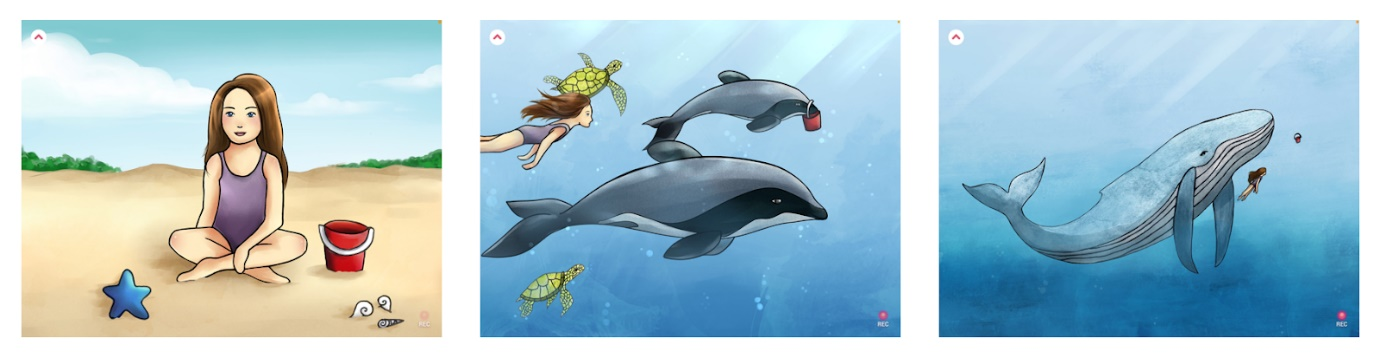
\includegraphics[width=\textwidth]{fig01.jpg}
 \caption{Ilustraciones de la historia seleccionada.}
 \label{fig01}
 \source{app \textit{Imagistory}.}
\end{figure}

\item[Fase II:] \textit{Diseño del instrumento de observación} para evaluar elnivel de autorregulación del aprendizaje del alumnado, siguiendo los constructos teóricos de \textcite{berridi_ramirez_estrategias_2017,requena_arellano_autorregulacion_2020}, e identificando dos dimensiones (\Cref{tbl01}).

\item[Fase III:]  \textit{Intervención} (abril-mayo 2021). Tras contar con la
autorización de participación de los menores, se les explicó la tarea arealizar con la app. Manipularon la aplicación individualmente durante10 minutos con la supervisión de una investigadora. Las locuciones
orales -junto con las ilustraciones de la app- se autograbaron en vídeos
de 3 minutos, visualizados posteriormente por el alumnado. La
investigadora no sólo los acompañó, sino que también realizó el
seguimiento y procedió al registro sistemático de lo observado durante
la actividad, utilizando una parrilla individualizada, como sugiere \textcite{anguera_metodologiobservacion_1978}.

\item[Fase IV] \textit{Análisis de las narraciones orales y tratamiento
estadístico de resultados.} Tres investigadores analizaron las
producciones orales (15 min/vídeo, 23h totales), atendiendo a los
indicadores recogidos en el instrumento. Posteriormente, se aplicaron
técnicas de análisis: frecuencias y porcentajes, medias (X) y desviación
típica (DT), así como medidas de asociación por medio de la correlación
de Pearson. Al no ajustarse la distribución de la muestra a la
normalidad respecto a las variables de clasificación de los sujetos, se
adoptaron las pautas adecuadas a este tipo de investigaciones -como indica \textcite{siegel_estadistica_2005}- empleando la prueba de Kolmogorov-Smirnov, los resultados en todos los casos fueron de $p < 0,001$. Los
contrastes de medias se realizaron con pruebas acordes al tipo de
variables: $U$ de Mann-Whitney para el género $y$ Kruskal-Wallis para el
resto, utilizando valores de $0,05$ para constatar la significatividad de
las diferencias. Se utilizó el programa SPSS-V27.
\end{description}


\section{Instrumento}\label{sec-instrumento}
El instrumento diseñado \emph{ad hoc} cumple los criterios de rigor al
obtener un destacado nivel de fiabilidad con un Alfa de Cronbach$=0,805$.
Permite analizar el nivel de \emph{autorregulación del aprendizaje} delalumnado a partir de la observación directa, adaptando los criterios de \textcite{berridi_ramirez_estrategias_2017,requena_arellano_autorregulacion_2020}. Consta de 10 indicadores
relativos a la tarea narrativa apoyada en la app, agrupados en dos dimensiones (\Cref{tbl01}):


\begin{table}[htpb]
\centering
\begin{threeparttable}
\caption{Dimensiones del Aprendizaje Autorregulado.}
\label{tbl01}
\begin{tabular}{p{0.4\textwidth}p{0.6\textwidth}}
\toprule
\multicolumn{2}{c}{Dimensión: Autonomía}\\
Variables & Categorías \\
\midrule
1. Nivel de autonomía inicial & 
Bajo: Necesita estímulo para iniciar la narración oral \newline
Medio: Se toma un tiempo para contextualizar la historia a partir de las ilustraciones \newline
Alto: Toma la iniciativa en la narración.
\\
2. Nivel de autonomía durante la tarea &
Bajo: Requiere feedback\newline
Medio: Necesita confirmación de su adecuación\newline
Alto: Muestra autonomía \\
\midrule
\multicolumn{2}{c}{Dimensión: Afectivo-emocional} \\
Variables & Categorías \\
\midrule
a) \textit{Interés} & \\
3. Interés durante la tarea narrativa \newline
4. Interés en el visionado posterior del relato &
Escala: 1=nada; 2=poco; 3=bastante; 4=mucho \\
b) \textit{Reacción afectiva} & \\
5. Empatía con los personajes\newline
6. Curiosidad \newline
7. Seguridad \newline
8. Disfrute\newline
9. Implicación en la historia\newline
10. Relación con sus vivencias personales &
Escala: 1=nada; 2=algo; 3=mucho \\
\bottomrule
\end{tabular}
\source{Elaboración propia.}
\notes{Se necessário, poderá ser adicionada uma nota ao final da tabela.}
\end{threeparttable}
\end{table}



\section{Resultados}
\subsection{Dimensión autonomía}
\subsubsection{Nivel de autonomía inicial}
La autonomía inicial de niños y niñas es semejante, pues en ambos casos la mayoría necesita algún estímulo para iniciar la narración. Además, las diferencias entre las medias (\Cref{tbl02}) -con la prueba $U$ de Mann-Whitney-, no son significativas ($p=0,229$). 

\begin{table}
\centering
\begin{threeparttable}
\caption{Descriptivos de la muestra respecto a la autonomía inicial y género.}
\label{tbl02}
\begin{tabular}{ll*{3}S}
\toprule
& & Niño & Niña & Total \\
\midrule
& N1: Necesita un estímulo para iniciar la narración & 72,92 & 60,00 & 66,67 \\
& N2: Se toma un tiempo para contextualizar la historia & 2,08 & 6,67 & 4,30 \\
& N3: Toma la iniciativa en la narración & 25,00 & 33,33 & 29,03 \\
\parbox[t]{2mm}{\multirow{3}{*}{\rotatebox[origin=c]{90}{Total}}}  & \% & 51,61 & 48,39 & 100,00 \\
& X & 1,52 & 1,73 & 1,62 \\
& DT & 0,87 & 0,93 & 0,90\\
\bottomrule
\end{tabular}
\source{Elaboración propia.}
\end{threeparttable}
\end{table}


A medida que aumenta la edad, el alumnado muestra mayor nivel de autonomía, necesita menos estímulos y presenta mayor iniciativa, salvo en el grupo de 6 años (\Cref{tbl03}), aunque la diferencia de medias -con la prueba de Kruskal-Wallis- no resulta significativa ($p=0,067$).


\begin{table}[htpb]
\centering
\begin{threeparttable}
\caption{Descriptivos de la muestra respecto a la autonomía inicial y edad.}
\label{tbl03}
\begin{tabular}{lp{0.4\textwidth}*{6}S}
\toprule
& & 4A & 4B & 5A & 5B & 6 & Total \\
\midrule
& N1: Necesita un estímulo para iniciar la narración & 100,00 & 70,83 & 65,00 & 48,15 & 76,92 & 66,67 \\
& N2: Se toma un tiempo para contextualizar la historia & 0,00 & 0,00 & 0,00 & 11,11 & 7,69 & 4,30 \\
& N3: Toma la iniciativa en la narración & 0,00 & 29,17 & 35,00 & 40,74 & 15,38 & 29,03 \\
\parbox[t]{2mm}{\multirow{3}{*}{\rotatebox[origin=c]{90}{Total}}} & \% & 9,68 & 25,81 & 21,51 & 29,03 & 13,98 & 100,00 \\
& X & 1,00 & 1,58 & 1,70 & 1,93 & 1,38 & 1,62 \\
& DT & 0,00 & 0,92 & 0,97 & 0,95 & 0,76 & 0,90 \\
\bottomrule
\end{tabular}
\source{Elaboración propia.}
\end{threeparttable}
\end{table}

Según el carácter, los sujetos introvertidos-tranquilos presentan menor autonomía inicial, aumentando en los extrovertidos-activos (\Cref{tbl04}). Tras contrastar las medias -con la prueba de Kruskal-Wallis- se corrobora que la autonomía inicial se incrementa al aumentar la extroversión, pues las diferencias son significativas ($p=0,019$).


\begin{table}[htpb]
\centering
\begin{threeparttable}
\caption{Descriptivos de la muestra respecto a la autonomía inicial y carácter.}
\label{tbl04}
\begin{tabular}{lp{0.4\textwidth}*{5}S}
\toprule
& & \text{Int/Tran} & \text{Int/Act} & \text{Ext/Tran} & \text{Ext/Act} & \text{Total} \\
\midrule
& N1: Necesita un estímulo para iniciar la narración & 80,00 & 77,78 & 63,16 & 46,15 & 66,67 \\
& N2: Se toma tiempo para contextualizar la historia & 6,67 & 5,56 & 5,26 & 0,00 & 4,30 \\
& N3: Toma la iniciativa en la narración & 13,33 & 16,67 & 31,58 & 53,85 & 29,03 \\
\parbox[t]{2mm}{\multirow{3}{*}{\rotatebox[origin=c]{90}{Total}}} & \% & 32,26 & 19,35 & 20,43 & 27,96 & 100,00 \\
& X & 1,33 & 1,39 & 1,68 & 2,08 & 1,62 \\
& DT & 0,71 & 0,77 & 0,94 & 1,01 & 0,90 \\
\bottomrule
\end{tabular}
\source{Elaboración propia.}
\end{threeparttable}
\end{table}

La autonomía inicial, independientemente del uso que hagan de la tableta los sujetos, es muy similar (\Cref{tbl05}), pues la mayoría necesita algún tipo de estímulo para iniciar la narración, y, en contra de lo que cabría esperar, los que no la usan presentan mayor iniciativa. Sin embargo, esa diferencia no resulta significativa al contrastar las medias con la prueba de Kruskal-Wallis ($p=0,324$). 


\begin{table}[htpb]
\centering
\begin{threeparttable}
\caption{Descriptivos de la muestra respecto a la autonomía inicial y uso de la tableta.}
\label{tbl05}
\begin{tabular}{lp{0.4\textwidth}*{4}S}
\toprule
& & \text{\begin{tabular}[c]{@{}l@{}}No tiene/\\No utiliza\end{tabular}} & \text{Ve vídeos} & \text{Juega} & \text{Total} \\
\midrule
& N1: Necesita estímulo para iniciar la narración & 58,06 & 68,75 & 73,33 & 66,67 \\
& N2: Toma tiempo para contextualizar la historia & 0,00 & 9,38 & 3,33 & 4,30 \\
& N3: Toma la iniciativa en la narración & 41,94 & 21,88 & 23,33 & 29,03 \\
\parbox[t]{2mm}{\multirow{3}{*}{\rotatebox[origin=c]{90}{Total}}} & \% & 33,33 & 34,41 & 32,26 & 100,0 \\
& \text{X} & 1,84 & 1,53 & 1,50 & 1,62 \\
& \text{DT} & 1,00 & 0,84 & 0,86 & 0,90 \\
\bottomrule
\end{tabular}
\source{Elaboración propia.}
\end{threeparttable}
\end{table}

El nivel de autonomía inicial aumenta en aquellos que presentan mayor nivel de destreza con la app, no de forma significativa aunque muy próxima a ella ($p=0,069$) (\Cref{tbl06}). 


\begin{table}[htpb]
\centering
\begin{threeparttable}
\caption{Descriptivos de la muestra respecto a la autonomía inicial y destreza con la app.}
\label{tbl06}
\begin{tabular}{lp{0.4\textwidth}*{4}S}
\toprule
& & \text{D1: Bajo} & \text{D2: Medio} & \text{D3: Alto} & \text{Total} \\
\midrule
& N1: Necesita un estímulo para iniciar la narración & 79,17 & 69,05 & 51,85 & 66,67 \\
& N2: Se toma tiempo para contextualizar la historia & 4,17 & 4,76 & 3,70 & 4,30 \\
& N3: Toma la iniciativa en la narración & 16,67 & 26,19 & 44,44 & 29,03 \\
\parbox[t]{2mm}{\multirow{3}{*}{\rotatebox[origin=c]{90}{Total}}} & \% & 25,81 & 45,16 & 29,03 & 100,0 \\
& \text{X} & 1,38 & 1,57 & 1,93 & 1,62 \\
& \text{DT} & 0,77 & 0,88 & 0,99 & 0,90 \\
\bottomrule
\end{tabular}
\source{Elaboración propia.}
\end{threeparttable}
\end{table}



\subsubsection{Autonomía durante la tarea}
La autonomía durante la tarea (73,12\%) (\Cref{tbl07}) es mayor que la inicial (29,03\%) independientemente del género (\Cref{tbl02}). Aparentemente, los niños se desenvuelven con mayor autonomía que las niñas, aunque las diferencias no resultan significativas ($p=0,182$). 

\begin{table}[htpb]
\centering
\begin{threeparttable}
\caption{Descriptivos de la muestra respecto a la autonomía durante la tarea y género.}
\label{tbl07}
\begin{tabular}{ll*{3}S}
\toprule
& & Niño & Niña & Total \\
\midrule
& N1: Requiere feedback para avanzar & 12,50 & 20,00 & 16,13 \\
& N2: Busca confirmación de su adecuación a la tarea & 8,33 & 13,33 & 10,75 \\
& N3: Muestra autonomía & 79,17 & 66,67 & 73,12 \\
\parbox[t]{2mm}{\multirow{3}{*}{\rotatebox[origin=c]{90}{Total}}} & \% & 51,61 & 48,39 & 100,00 \\
& X & 2,67 & 2,47 & 2,57 \\
& DT & 0,694 & 0,815 & 0,758 \\
\bottomrule
\end{tabular}
\source{Elaboración propia.}
\end{threeparttable}
\end{table}


Al igual que sucede con la autonomía inicial del alumnado (\Cref{tbl07}), la autonomía durante la tarea se incrementa con la edad, menos en 6 años (\Cref{tbl08}), aunque no significativamente ($p=0,134$).


\begin{table}[htpb]
\centering
\begin{threeparttable}
\caption{Descriptivos de la muestra respecto a la autonomía durante la tarea y edad.}
\label{tbl08}
\begin{tabular}{lp{0.4\textwidth}*{6}S}
\toprule
& & \text{4A} & \text{4B} & \text{5A} & \text{5B} & \text{6} & \text{Total} \\
\midrule
& N1: Requiere feedback para avanzar & 44,44 & 16,67 & 15,00 & 3,70 & 23,08 & 16,13 \\
& N2: Busca confirmación de su adecuación a la tarea & 0,00 & 4,17 & 15,00 & 11,11 & 23,08 & 10,75 \\
& N3: Muestra autonomía & 55,56 & 79,17 & 70,00 & 85,19 & 53,85 & 73,12 \\
\parbox[t]{2mm}{\multirow{3}{*}{\rotatebox[origin=c]{90}{Total}}} & \% & 9,68 & 25,81 & 21,51 & 29,03 & 13,98 & 100,0 \\
& X & 2,11 & 2,63 & 2,55 & 2,81 & 2,31 & 2,57 \\
& DT & 1,05 & 0,77 & 0,75 & 0,48 & 0,85 & 0,75 \\
\bottomrule
\end{tabular}
\source{Elaboración propia.}
\end{threeparttable}
\end{table}

Se constata que el grado de autonomía durante la tarea narrativa se incrementa a medida que crece el nivel de extroversión ($p=0,019$) (Tabla 9).



\begin{table}[htpb]
\centering
\begin{threeparttable}
\caption{Descriptivos de la muestra respecto a la autonomía durante la tarea y carácter.}
\label{tbl09}
\begin{tabular}{lp{0.4\textwidth}*{5}S}
\toprule
& & \text{Int/Tran} & \text{Int/Act} & \text{Ext/Tran} & \text{Ext/Act} & \text{Total} \\
\midrule
& N1: Requiere feedback para avanzar & 30,00 & 5,56 & 21,05 & 3,85 & 16,13 \\
& N2: Busca confirmación de su adecuación a la tarea & 13,33 & 16,67 & 10,53 & 3,85 & 10,75 \\
& N3: Muestra autonomía & 56,67 & 77,78 & 68,42 & 92,31 & 73,12 \\
\parbox[t]{2mm}{\multirow{3}{*}{\rotatebox[origin=c]{90}{Total}}} & \% & 32,26 & 19,35 & 20,43 & 27,96 & 100,00 \\
& X & 2,27 & 2,72 & 2,47 & 2,88 & 2,57 \\
& DT & 0,90 & 0,57 & 0,84 & 0,43 & 0,75 \\
\bottomrule
\end{tabular}
\source{Elaboración propia.}
\end{threeparttable}
\end{table}

El alumnado con mayor autonomía durante la tarea coincide con aquel que usa la tableta para jugar (\Cref{tbl10}), aunque esas diferencias no son significativas ($p=0,789$).



\begin{table}[htpb]
\centering
\begin{threeparttable}
\caption{Descriptivos de la muestra respecto a la autonomía durante la tarea y uso de la tableta.}
\label{tbl10}
\begin{tabular}{lp{0.4\textwidth}*{4}S}
\toprule
& & \text{\begin{tabular}[c]{@{}l@{}}No tiene/\\No usa\end{tabular}} & \text{Ve vídeos} & \text{Juega} & \text{Total} \\
\midrule
& N1: Requiere feedback para avanzar & 16,13 & 15,63 & 16,67 & 16,13 \\
& N2: Busca confirmación de su adecuación a la tarea & 16,13 & 9,38 & 6,67 & 10,75 \\
& N3: Muestra autonomía & 67,74 & 75,00 & 76,67 & 73,12 \\
\parbox[t]{2mm}{\multirow{3}{*}{\rotatebox[origin=c]{90}{Total}}} & \% & 33,33 & 34,41 & 32,26 & 100,0 \\
& X & 2,52 & 2,59 & 2,60 & 2,57 \\
& DT & 0,76 & 0,75 & 0,77 & 0,75 \\
\bottomrule
\end{tabular}
\source{Elaboración propia.}
\end{threeparttable}
\end{table}


La autonomía durante la tarea tampoco se relaciona con el nivel de destreza con la app del alumnado al no resultar significativo ($p=0,666$) (\Cref{tbl11}).



\begin{table}[htpb]
\centering
\begin{threeparttable}
\caption{Descriptivos de la muestra: autonomía durante la tarea y destreza con la app.}
\label{tbl11}
\begin{tabular}{lp{0.4\textwidth}*{4}S}
\toprule
& & \text{D1: Baja} & \text{D2: Media} & \text{D3: Alta} & \text{Total} \\
\midrule
& N1: Requiere feedback para avanzar & 12,50 & 19,05 & 14,81 & 16,13 \\
& N2: Busca confirmación de su adecuación a la tarea & 8,33 & 11,90 & 11,11 & 10,75 \\
& N3: Muestra autonomía & 79,17 & 69,05 & 74,07 & 73,12 \\
\parbox[t]{2mm}{\multirow{3}{*}{\rotatebox[origin=c]{90}{Total}}} & \% & 25,81 & 45,16 & 29,03 & 100,00 \\
& X & 2,67 & 2,50 & 2,59 & 2,57 \\
& DT & 0,70 & 0,80 & 0,74 & 0,75\\
\bottomrule
\end{tabular}
\source{Elaboración propia.}
\end{threeparttable}
\end{table}


\subsection{Dimensión afectivo-emocional}
\subsubsection{Interés}

Las diferencias entre el interés manifestado por niños y niñas no son significativas ni durante ($p=0,237$) ni después ($p=0,085$), aunque estas muestran algo más de interés durante la tarea narrativa y en el posterior visionado de su relato oral (\Cref{tbl12}).

\begin{table}[htpb]
\centering
\begin{threeparttable}
\caption{Descriptivos de la muestra respecto al interés mostrado y género.}
\label{tbl12}
\begin{tabular}{ll*{6}S}
\toprule
& & \multicolumn{3}{c}{Durante la tarea narrativa} & \multicolumn{3}{p{4cm}}{En el posterior visionado del relato} \\
& & Niño & Niña & Total & Niño & Niña & Total \\
\midrule
\multicolumn{2}{l}{(1) Nada} & 10,42 & 0,00 & 5,43 & 14,58 & 6,67 & 10,75 \\
\multicolumn{2}{l}{(2) Poco} & 22,92 & 27,27 & 25,00 & 33,33 & 22,22 & 27,96 \\
\multicolumn{2}{l}{(3) Bastante} & 45,83 & 43,18 & 44,57 & 20,83 & 28,89 & 24,73 \\
\multicolumn{2}{l}{(4) Mucho} & 20,83 & 29,55 & 25,00 & 31,25 & 42,22 & 36,56 \\
\parbox[t]{2mm}{\multirow{3}{*}{\rotatebox[origin=c]{90}{Total}}} & \% & 52,17 & 47,83 & 100,0 & 51,61 & 48,39 & 100,0 \\
& \text{X} & 2,77 & 3,02 & 2,89 & 2,69 & 3,07 & 2,87 \\ 
& \text{DT} & 0,90 & 0,76 & 0,84 & 1,07 & 0,96 & 1,03 \\
\bottomrule
\end{tabular}
\source{Elaboración propia.}
\end{threeparttable}
\end{table}

De forma semejante, el interés mostrado por el alumnado durante la tarea, atendiendo a la edad, no arroja diferencias significativas ($p=0,275$), como tampoco lo hace en el posterior visionado ($p=0,693$). En cambio, en cuanto al carácter, se observa que a medida que aumenta la extroversión se incrementa significativamente el interés tanto durante la tarea narrativa ($p=0,01$) como en el posterior visionado de su relato oral ($p=0,006$). La \Cref{fig02} ofrece la progresión lineal entre ambas variables atendiendo a las medias. 

\begin{figure}[htbp] \centering 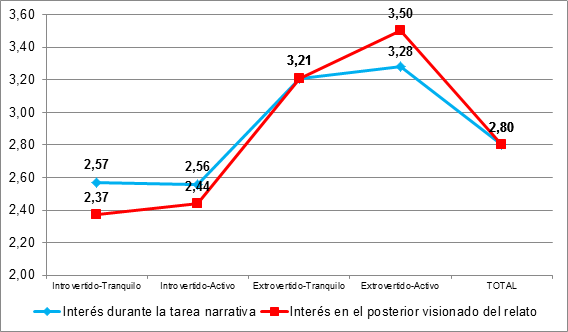
\includegraphics[width=0.75\textwidth]{fig02.png}
 \caption{Progresión de las medias respecto al interés y carácter.}
 \label{fig02}
 \source{elaboración propia.}
\end{figure}

Por contra, el interés del alumnado no se relaciona significativamente con el uso que hacen de la tableta, ni durante la tarea ($p=0,479$) ni en el posterior visionado de su relato oral ($p=0,679$). Sin embargo, en cuanto al nivel de destreza con la app, se comprueba que a medida que este es mayor aumenta el nivel de interés durante la tarea narrativa ($p=0,023$), aunque no así respecto al visionado posterior ($p=0,359$).

Se observa que los sujetos que no saben interaccionar con la app (D1) muestran mayor interés en el visionado posterior de su relato oral, al contrario que los que tienen mayor nivel de destreza (\Cref{tbl13}).

\begin{table}[htpb]
\centering
\begin{threeparttable}
\caption{Medias y desviación típica del interés mostrado y destreza con la app.}
\label{tbl13}
\begin{tabular}{l*{4}S}
\toprule
Interés & \multicolumn{2}{c}{Durante la narración} & \multicolumn{2}{p{3cm}}{En el posterior visionado del relato} \\
\midrule
Destreza con la app & \text{X} & \text{DT} & X & \text{DT} \\
D1. Baja & 2,48 & 0,94 & 2,67 & 1,23 \\
D2. Media & 2,93 & 0,77 & 2,83 & 0,96 \\
D3. Alta & 3,19 & 0,73 & 3,11 & 0,93 \\
Total & 2,89 & 0,84 & 2,87 & 1,03 \\
\bottomrule
\end{tabular}
\source{Elaboración propia.}
\end{threeparttable}
\end{table}



\subsubsection{Reacción afectiva}

El alumnado muestra gran seguridad al narrar oralmente su historia (\Cref{tbl14}), aunque empatiza poco con los personajes del relato y apenas establece relación con sus experiencias personales. Se observa que las niñas presentan valores más altos en la mayoría de las variables afectivas.


\begin{table}[htpb]
\centering
\begin{threeparttable}
\caption{Media y desviación típica de las variables afectivas y género.}
\label{tbl14}
\begin{tabular}{l*{6}S}
\toprule
 & \multicolumn{2}{c}{Niño} & \multicolumn{2}{c}{Niña} & \multicolumn{2}{c}{Total} \\
 & \text{X} & \text{DT} & \text{X} & \text{DT} & \text{X} & \text{DT} \\
\midrule
Empatiza con los personajes & 1,42 & 0,61 & 1,78 & 0,76 & 1,59 & 0,71 \\
Manifiesta curiosidad & 1,94 & 0,59 & 2,22 & 0,67 & 2,08 & 0,64 \\
Muestra seguridad & 2,75 & 0,56 & 2,73 & 0,58 & 2,74 & 0,56 \\
Disfruta de la narración & 2,08 & 0,73 & 2,27 & 0,72 & 2,17 & 0,73 \\
Se sumerge en el relato & 1,94 & 0,78 & 2,02 & 0,83 & 1,98 & 0,80 \\
Relaciona el relato con sus vivencias personales & 1,15 & 0,50 & 1,02 & 0,14 & 1,09 & 0,38 \\
\bottomrule
\end{tabular}
\source{Elaboración propia.}
\end{threeparttable}
\end{table}

Esta tendencia se confirma al correlacionar el género con las variables afectivas -(1=niños y 2=niñas), obteniendo una correlación positiva significativa (\Cref{tbl15}), lo que indica que la reacción afectiva es más alta en ellas; concretamente, las niñas muestran mayor curiosidad y empatía con los personajes del relato. 

\begin{table}[htpb]
\centering
\begin{threeparttable}
\caption{Correlación de Pearson: variables afectivas y género ($N=93$).}
\label{tbl15}
\begin{tabular}{llS}
\toprule
 & & \text{Género} \\
\midrule
Empatiza con los personajes & Correlación de Pearson & 0,255* \\
 & Sig. (bilateral) & 0,014 \\
Manifiesta curiosidad & Correlación de Pearson & 0,221* \\
 & Sig. (bilateral) & 0,033 \\
Muestra seguridad & Correlación de Pearson & -0,015 \\
 & Sig. (bilateral) & 0,889 \\
Disfruta de la narración & Correlación de Pearson & 0,126 \\
 & Sig. (bilateral) & 0,229 \\
Se sumerge en el relato & Correlación de Pearson & 0,053 \\
 & Sig. (bilateral) & 0,616 \\
Relaciona el relato con sus vivencias personales & Correlación de Pearson & -0,163 \\
 & Sig. (bilateral) & 0,118 \\
\bottomrule
\end{tabular}
\source{Elaboración propia.}
\notes{** La correlación es significativa en el nivel 0,01 (bilateral). * La correlación es significativa en el nivel 0,05 (bilateral).}
\end{threeparttable}
\end{table}

No hay diferencias significativas respecto a los grupos etarios, observándose una gran homogeneidad (\Cref{tbl16}).



\begin{table}[htpb]
\centering
\begin{threeparttable}
\caption{Estadísticos descriptivos de las variables afectivas y la edad.}
\label{tbl16}
\begin{tabular}{ p{2cm} *{12}{S[table-format = 1.2]} }
\toprule
 & \multicolumn{2}{c}{4A} & \multicolumn{2}{c}{4B} & \multicolumn{2}{c}{5A} & \multicolumn{2}{c}{5B} & \multicolumn{2}{c}{6} & \multicolumn{2}{c}{Total}\\
 & \text{X} & \text{DT} & \text{X} & \text{DT} & \text{X} & \text{DT} & \text{X} & \text{DT} & \text{X} & \text{DT} & \text{X} & \text{DT} \\
\midrule
Empatiza con personajes & 1,22 & 0,44 & 1,79 & 0,77 & 1,40 & 0,59 & 1,70 & 0,72 & 1,54 & 0,77 & 1,59 & 0,71 \\
Manifiesta curiosidad & 2,00 & 0,50 & 2,13 & 0,61 & 1,90 & 0,64 & 2,30 & 0,60 & 1,85 & 0,80 & 2,08 & 0,64 \\
Muestra seguridad & 2,44 & 0,72 & 2,88 & 0,44 & 2,75 & 0,63 & 2,85 & 0,36 & 2,46 & 0,77 & 2,74 & 0,56 \\
Disfruta de la narración & 1,89 & 0,78 & 2,21 & 0,58 & 2,05 & 0,75 & 2,37 & 0,74 & 2,08 & 0,86 & 2,17 & 0,73 \\
Se sumerge en el relato & 1,56 & 0,72 & 1,96 & 0,80 & 1,80 & 0,69 & 2,30 & 0,77 & 1,92 & 0,95 & 1,98 & 0,80 \\
Relaciona el relato con vivencias personales & 1,00 & 0,00 & 1,00 & 0,00 & 1,15 & 0,48 & 1,11 & 0,42 & 1,15 & 0,55 & 1,09 & 0,38 \\
\bottomrule
\end{tabular}
\source{Elaboración propia.}
\end{threeparttable}
\end{table}

En cuanto al carácter, al contrastar las medias -con la prueba Kruskal-Wallis-, se constata que las personas más extrovertidas manifiestan significativamente más curiosidad ($p=0,021$), disfrute con la historia ($p=0,001$) e inmersión en el relato oral ($p=0,004$). Por tanto, se puede afirmar que la reacción afectiva aumenta a medida que se incrementa el nivel de extroversión (\Cref{tbl17}).


\begin{table}[htpb]
\centering
\begin{threeparttable}
\caption{Medias y desviación típica: reacción afectiva según el carácter.}
\label{tbl17}
\begin{tabular}{ p{3cm} *{10}{S[table-format = 1.2]} }
\toprule
 & \multicolumn{2}{c}{Int/Tran} & \multicolumn{2}{c}{Int/Act} & \multicolumn{2}{c}{Ext/Tran} & \multicolumn{2}{c}{Ext/Act} & \multicolumn{2}{c}{Total} \\
 & \text{X} & \text{DT} & \text{X} & \text{DT} & \text{X} & \text{DT} & \text{X} & \text{DT} & \text{X} & \text{DT}  \\
\midrule
Empatiza con los personajes & 1,40 & 0,49 & 1,56 & 0,78 & 1,63 & 0,76 & 1,81 & 0,80 & 1,59 & 0,71 \\
Manifiesta curiosidad & 1,90 & 0,60 & 1,89 & 0,67 & 2,11 & 0,65 & 2,38 & 0,57 & 2,08 & 0,64 \\
Muestra seguridad & 2,67 & 0,60 & 2,61 & 0,60 & 2,74 & 0,65 & 2,92 & 0,39 & 2,74 & 0,56 \\
Disfruta de la narración & 1,87 & 0,68 & 2,06 & 0,72 & 2,16 & 0,68 & 2,62 & 0,63 & 2,17 & 0,73 \\
Se sumerge en el relato & 1,70 & 0,75 & 1,72 & 0,75 & 2,05 & 0,84 & 2,42 & 0,70 & 1,98 & 0,80 \\
Relaciona el relato con sus vivencias personales & 1,03 & 0,18 & 1,00 & 0,00 & 1,21 & 0,63 & 1,12 & 0,43 & 1,09 & 0,38 \\
\bottomrule
\end{tabular}
\source{Elaboración propia.}
\end{threeparttable}
\end{table}

La reacción afectiva aumenta progresivamente a medida que poseen mayor destreza (\Cref{fig03}), aunque las variables afectivas no se relacionan con el uso de la tableta, pues el contraste de medias -efectuado con la prueba de Kruskal-Wallis- presenta valores $p > 0,05$ para todas ellas. Solo son significativas respecto al disfrute con el relato oral que manifiestan ($p=0,006$) y a la inmersión en él ($p=0,018$).

\begin{figure}[htbp] \centering 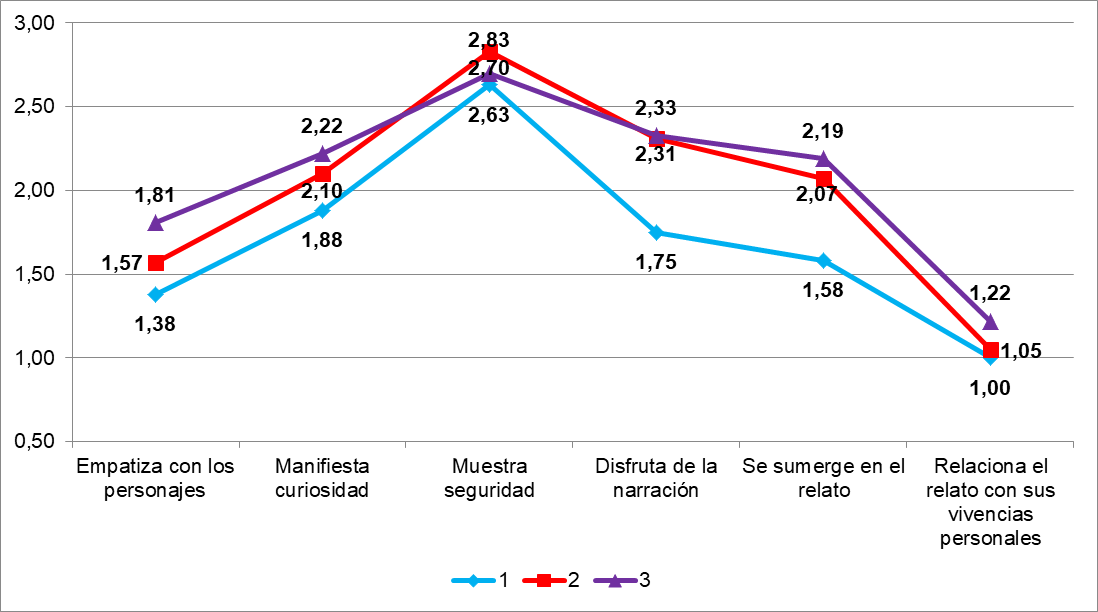
\includegraphics[width=0.75\textwidth]{fig03.png}
 \caption{Progresión entre las variables afectivas y el nivel de destreza con la app.}
 \label{fig03}
 \source{elaboración propia.}
\end{figure}

La actividad de narración oral con apoyo de la app seleccionada ha incrementado la autonomía del alumnado de Educación Infantil durante la tarea, así como su motivación ligada al interés y curiosidad suscitada. Asimismo, la experiencia narrativa auxiliada en la app ha afianzado su seguridad en la tarea, inmersión y disfrute con el relato oral. Por ende, ha contribuido a favorecer su autorregulación del aprendizaje.

\section{Discusión y conclusiones}

El nivel de autonomía inicial del alumnado frente a la tarea narrativa apoyada en la app es bajo, pues la mayoría necesita algún estímulo para iniciar su propia narración oral a partir de las ilustraciones de la app. Posiblemente, muchos están acostumbrados a escuchar relatos, pero no a narrarlos espontáneamente -como se les propuso en este estudio-. Sin embargo, a medida que se implican en la tarea su autonomía se incrementa, debido a que van interiorizando la actividad solicitada y calibrando el nivel de dificultad que implica. Las directrices enunciadas al inicio por la investigadora resultaron clave para que aprendieran a secuenciar y construir tramas a partir de las imágenes, como reconocen \textcite{torremocha_libros_2002}.

En general, se observa el aumento de la autorregulación del aprendizaje a medida que avanza la edad, pues se trata de un periodo de desarrollo madurativo sujeto a distintos ritmos. El uso que hacen de la tableta y la destreza con la app no condiciona su nivel de autorregulación del aprendizaje por tratarse de una actividad idónea para este alumnado, al no exigir experiencia previa, aunque tiende a aumentar en aquellos acostumbrados a manejar este dispositivo.

Se observa que quienes poseen mayor nivel de destreza con la app disfrutan más interaccionando con esta, aunque menos con el visionado posterior del relato oral. El alumnado que se siente más seguro al utilizar la app muestra mayor interés por la tarea. No ocurre lo mismo con el posterior visionado y escucha, lo cual podría deberse a la timidez ocasionada al escuchar su propia voz. Además, curiosamente, los que presentan menor destreza con la app manifiestan más interés por ver el resultado final.

Al igual que \textcite{bertolini_theory_2017}, se constata que la interacción con la app incrementa el interés del alumnado. En este estudio, son los extrovertidos quienes tienen mayor interés para elaborar las narraciones orales, a diferencia de los introvertidos, que se sienten más cohibidos y muestran mayor timidez al escuchar su propia voz. Esta tarea puede ser beneficiosa para reforzar la autoestima y enseñar que el error es una fuente de aprendizaje desde edades tempranas \cite{cepa_serrano_educacion_2017}. Por su parte, en cuanto a la reacción afectiva, las niñas muestran mayor curiosidad y empatía con los personajes, lo que quizá pueda relacionarse con que la protagonista de la historia es una niña, facilitando su proyección. Por ello, se requiere la creación de relatos ilustrados con personajes y tramas diversas que permitan establecer mayor empatía con los personajes y vincularlos con sus vivencias personales.

Cabe destacar que las relaciones más significativas se observan entre la variable carácter del alumnado y las dimensiones autonomía y afectivo-emocional, de ahí la importancia de impulsar la educación emocional desde edades tempranas y diseñar actividades que estimulen la empatía, el respeto, la autoestima, el reconocimiento y la expresión emocional propia y ajena, así como las habilidades comunicativas en su conjunto, pues estas influyen en la autorregulación del aprendizaje y en procesos cognitivos complejos \cite{bocci_apps_2017,ramya_gangaiamaran_review_2017}. Dada la importancia de la implicación emocional en el aprendizaje y, en particular, en las tareas de producción lingüística, sería conveniente diseñar estrategias narrativas para potenciar una mayor respuesta emocional del alumnado. Por ejemplo, visionar y comentar en el aula las ilustraciones antes de grabar el relato digital podría favorecer su implicación afectiva.

Evidentemente, esta app ha favorecido el desarrollo de habilidades de lectura e interpretación de imágenes, como subrayan \textcite{leon_review_2017} tras una experiencia similar. La práctica regular de relatos digitales de forma oral podría aportarles mayor seguridad, especialmente a los más introvertidos. Además, la reiterada utilización de la app facilitaría un ágil manejo, pudiendo mejorar su autorregulación del aprendizaje, referido en este caso a la tarea narrativa espontánea.

Es interesante aprovechar el potencial motivador y lúdico de las app para integrarlas en Educación Infantil, pues su fácil manejo fomenta la autonomía para acometer la tarea narrativa apoyada en ilustraciones. Así pues, este tipo de app puede resultar motivadora y atractiva para el alumnado al estar familiarizado con estas herramientas digitales para jugar o ver vídeos. También es inclusiva con el Alumnado con Necesidades Específicas de Apoyo Educativo (ACNEAE), pues consta de una interfaz sencilla que permite la asimilación de tareas complejas al igual que señalan \textcite{jimenez_utilizacion_2017}. Adicionalmente, no solo contribuye a favorecer la autorregulación del aprendizaje -activando la autonomía-, el interés y la reacción afectiva del alumnado desde las primeras edades, sino que también puede resultar útil para evaluar dichos aspectos. Además, al no existir diferencias significativas entre el alumnado que dispone de tableta y el que no, se deduce que la utilización previa de esta no es un hándicap que dificulte el desarrollo de estas habilidades.

Cabe destacar la adecuación de la aplicación utilizada, pues, independientemente de la edad, género o familiarización previa con el manejo de tabletas, resulta idónea para desarrollar narraciones orales en el aula en cualquiera de los tres cursos del segundo ciclo de Educación Infantil. Finalmente, dada la escasez de investigaciones vinculadas al desarrollo de la autorregulación del aprendizaje con este tipo de app en Educación Infantil, sería pertinente realizar más estudios similares ampliando la muestra y explorando otras app para contrastar los resultados.


\printbibliography\label{sec-bib}
% if the text is not in Portuguese, it might be necessary to use the code below instead to print the correct ABNT abbreviations [s.n.], [s.l.]
%\begin{portuguese}
%\printbibliography[title={Bibliography}]
%\end{portuguese}


%full list: conceptualization,datacuration,formalanalysis,funding,investigation,methodology,projadm,resources,software,supervision,validation,visualization,writing,review
\begin{contributors}[sec-contributors]
\authorcontribution{María Esther del-Moral Pérez}[conceptualization,investigation,datacuration,investigation,methodology,projadm,writing]
\authorcontribution{Nerea López-Bouzas}[conceptualization,investigation,datacuration,investigation,methodology,writing]
\authorcontribution{Jonathan Castañeda Fernández}[investigation,formalanalysis,datacuration,methodology,validation,writing]
\authorcontribution{María del Rosario Neira-Piñeiro}[conceptualization,investigation,datacuration,investigation,methodology,writing]
\end{contributors}





\end{document}

